

\documentclass[11pt,a4paper]{scrartcl}
\typearea{12}
\usepackage{graphicx}
%\usepackage{pstricks}
\usepackage{listings}
\usepackage{color}
\usepackage{tikz}
\usetikzlibrary{decorations.markings}
\lstset{language=C}
\usepackage{fancyhdr}
\pagestyle{fancy}
\begin{document}

\section*{Worksheet 7}


\begin{center}
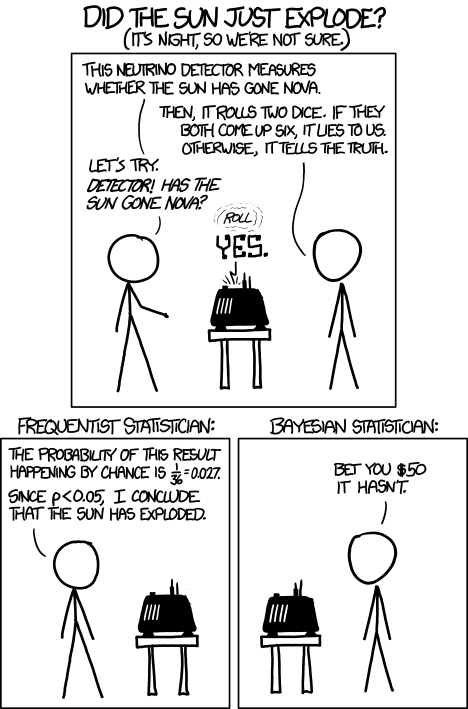
\includegraphics[width=7.5cm]{frequentists_vs_bayesians.png}
\end{center}
\texttt{https://xkcd.com/1132/}. It is also worth reading Randall Monroe's comment on the response to this cartoon:

\begin{quote}
Hey! I was kinda blindsided by the response to this comic.

I'm in the middle of reading a series of books about forecasting
errors (including N*** S***'s book, which I really enjoyed), and
again and again kept hitting examples of mistakes caused by blind
application of the textbook confidence interval approach.

Someone asked me to explain it in simple terms, but I realized that in
the common examples used to illustrate this sort of error, like the
cancer screening/drug test false positive ones, the correct result is
surprising or unintuitive. So I came up with the sun-explosion
example, to illustrate a case where na\"ive application of that
significance test can give a result that's obviously nonsense.

I seem to have stepped on a hornet's nest, though, by adding
`Frequentist' and `Bayesian' titles to the panels. This came as a
surprise to me, in part because I actually added them as an
afterthought, along with the final punchline. (I originally had the
guy on the right making some other cross-panel comment, but I thought
the `bet' thing was cuter.)

The truth is, I genuinely didn't realize Frequentists and Bayesians
were actual camps of people, all of whom are now emailing me. I thought
they were loosely-applied labels, perhaps just labels appropriated by
the books I had happened to read recently, for the standard textbook
approach we learned in science class versus an approach which more
carefully incorporates the ideas of prior probabilities.

I meant this as a jab at the kind of shoddy misapplications of
statistics I keep running into in things like cancer screening (which
is an emotionally wrenching subject full of poorly-applied
probability) and political forecasting. I wasn't intending to
characterize the merits of the two sides of what turns out to be a
much more involved and ongoing academic debate than I realized.

A sincere thank you for the gentle corrections; I've taken them to
heart, and you can be confident I will avoid such mischaracterizations
in the future!

At least, 95.45\% confident.
\end{quote}

\subsection*{Useful facts}

\begin{itemize}


\item The \textbf{conditional probability} of event $R$ given $C$:
  \begin{equation}
P(R|C)=\frac{P(R\cap C)}{P(C)} 
  \end{equation}
  This is the probability of getting an outcome in event $R$ if we
  know the outcome is in event $C$.

\item \textbf{Independence}: two events $A$ and $B$ are \textbf{independent} iff
  \begin{equation}
    P(A\cap B)=P(A)P(B)
  \end{equation}
  They are \textbf{conditionally independent}, given $C$, iff
  \begin{equation}
    P(A\cap B|C)=P(A|C)P(B|C)
  \end{equation}

\item \textbf{Bayes's rule}
\begin{equation}
P(A|B)=\frac{P(B|A)P(A)}{P(B)}
\end{equation}


\item  Here I use set notation for events, this is one approach, sometimes people prefer logic notation, even when the set notation is strictly correct!
 \textbf{Set notation}:
  \begin{itemize}
\item The bar `$|$' in sets should be read as `such that', so $A=\{x|\mbox{some stuff}\}$ should be read as $A$ is the set of $x$ \textbf{such that} `some stuff' is true and $A=\{x\in \mathbf{Z}|x>3\mbox{ and }x<10\}$ is the set $A=\{4,5,6,7,8,9\}$. $\mathbf{Z}$ by the way is the set of integers.
  \item $A\cup B$ is the union so $A\cup B=\{x|x\in A\mbox{ or }x\in B\}$. If $A=\{1,2,3\}$ and $B=\{3,4,5\}$ then $A\cup B=\{1,2,3,4,5\}$
  \item $A\cap B$ is the intersection so $A\cap B=\{x|x\in A\mbox{ and }x\in B\}$. If $A=\{1,2,3\}$ and $B=\{3,4,5\}$ then $A\cup B=\{3\}$
   \item $A\setminus B$ is the set minus so $A\setminus B=\{x|x\in A\mbox{ and }x\not\in B\}$. If $A=\{1,2,3,4\}$ and $B=\{1,3,5\}$ then $A\setminus B=\{2,4\}$
   \item If $C$ is a subset, the complement of $C$, that is the set of all the elements not in $C$, is written $\bar{C}$. If $X=\{1,2,3,4\}$ and $C=\{1,2\}$ then $\bar{C}=\{3,4\}$.
  \end{itemize}
  For events, $A\cup B$ is the event of $A$ or $B$ happening, $A\cap
  B$ is the event of $A$ and $B$ happening, $A\setminus B$ is the
  event of $A$ happening but $B$ not happening and $\bar{C}$ is the
  event of $C$ not happening.

  \end{itemize}

\subsection*{Questions}


\begin{enumerate}

\item Two events $A$ and $B$ have probabilities $P(A)=0.2$, $P(B)=0.3$ and $P(A\cup B)=0.4$. Find
\begin{enumerate}
\item Find $P(A\cap B)$.
\item Find $P(\bar{A}\cap \bar{B})$.
\item Find $P(A|B)$.
\end{enumerate}

\item In a library where all books have blue or yellow spines, four
  fifths of books with yellow spines are about mathematics but only a
  fifth of books with blue spines are about mathematics. There are the
  same number of yellow and blue spined books, you come upom a book
  open on a table; the book is about mathematics. What is the chance
  it has a yellow spine?

\item You want to go for a walk. However, when you wake up the day is
  cloudy and half of all raining days start off cloudy. On the other
  hand, two days in five start off cloudy and it's been rather dry
  recently with only rain only on one day in ten. What is the chance
  it will rain?
  
\item One night in a bar in Las Vegas you meet a dodgy character who
  tells you that there are two types of slot machine in the Topicana,
  one that pays out 10\% of the time, the other 20\%. One sort of
  machine is blue, the other red. Unfortunately the dodgy character is
  too drunk to remember which is which. The next day you randomly
  select red to try, you find a red machine and put in a coin. You
  lose. Assuming the dodgy character was telling the truth, what is
  the chance the red machine is the one that pays out more. If you had
  won instead of losing, what would the chance be?\footnote{I stole
    this problem from \texttt{courses.smp.uq.edu.au/MATH3104/}}
  
\item In the xkcd cartoon above, what is the chance the Bayesian will
  win his or her bet if the chance the sun has exploded is one in a
  million? In reality the chance is, of course, much less than one in
  a million! Show the answer to six decimal places.
  
\end{enumerate}
\end{document}

